\documentclass[bachelor]{ctexart}
\usepackage{hyperref}
\usepackage{geometry}
\usepackage{graphicx}
%\geometry{a4paper,scale=0.8}
%\geometry{a4paper,left=2cm,right=2cm,top=3cm,bottom=4cm}
\usepackage{fancyhdr}
\pagestyle{fancy}
\lhead{}
\chead{}
\rhead{\bfseries    学号       姓名}
\title{HOMEWORK 2}
\author{姓名}
\begin{document}
\maketitle
一、问题概述:

1) Please build a Gaussian mixture model (GMM) to model the data in file {TrainingData\_GMM.csv}. Note that the data is composed of 4 clusters, and the model should be trained by expectation maximization (EM) algorithm

2) Based on the GMM learned above, assign each training data point into one of 4 different clusters

二、报告要求:

1) Show how the log-likelihood evolves as the training proceeds

2) The learned mathematical expression for the GMM model after training on the given dataset

3) Randomly select 500 data points from the given dataset and plot them on a 2-dimensional coordinate system. Mark the data points coming from the same cluster (using the results of Problem 2) with the same color.

4) Some analyses on the impacts of initialization on the converged values of EM algorithm

5) Some analyses on the results you obtained

三、问题分析

本次实验的主要核心问题为使用GMM模型来拟合训练数据,使用EM算法来优化GMM模型中的参数。

1)高斯混合模型(GMM)

设随机变量\textbf{X},则混合高斯模型可用如下表示:
\begin{equation}
p(x) = \sum_{k=1}^{K}\pi_k N(\textbf{x}|\mu_k, {\sum}_k)
\end{equation}
其中$N(\textbf{x}|\mu_k, {\sum}_k)$为混合模型的第$k$个分量,$K$为总的总的模型数量,在本题中$K=4$.$\pi_k$为混合系数,满足
\begin{equation}
\sum_{k=1}^{K}\pi_k = 1, 0 \leq \pi_k \leq 1
\end{equation}

2)EM算法估计GMM参数

EM算法分为两步,第一步首先估计参数的粗略值,第二部使用第一步的值最大化似然函数。首先求出GMM的似然函数。

假设$\textbf{X} = \{\textbf{x}_1, \textbf{x}_2, \textbf{x}_N\}$,$X$是训练数据中所有的点,在本题中$N=5000$且每个点的维数为2.(1)式可写为:
\begin{equation}
p(x|\pi, \mu, \sum) = \sum_{k=1}^{K}\pi_k N(\textbf{x}|\mu_k, {\sum}_k)
\end{equation}

为了上述三个参数,需要分别求解出这三个参数的最大似然函数。首先求出$\mu_k$的最大似然函数。上式对$\mu_k$求导并令其导数为0得到:
\begin{equation}
0 = - \sum_{n=1}^{N}\frac{\pi_kN(\textbf{x}_n|\mu_k, {\sum}_k)}{\sum\limits_{j=1}^{N}\pi_jN(\textbf{x}_n|\mu_j, {\sum}_j)}{\sum}_k(\textbf{x}_n - \mu_k)
\end{equation}

\begin{equation}
\mu_k = \frac{1}{N_k}\sum_{n=1}^{K}\gamma(z_{nk})\textbf{x}_n
\end{equation}
其中$N_k = \sum_{n=1}^{N}\gamma(z_{nk})$.而$\gamma(z_{nk})$表示$\textbf{x}_n$属于聚类$k$的后验概率。

\begin{equation}
\gamma(z_k) = p(z_k = 1|\textbf{x})\\
 = \frac{\pi_k N(\textbf{x}|\mu_k, {\sum}_k)}{\sum\limits_{j = 1}^{K} \pi_j N(\textbf{x}|\mu_j, {\sum}_j)}
\end{equation}

同理可得
\begin{equation}
{\sum}_k = \frac{1}{N_k}\sum_{n=1}^{N}\gamma(z_nk)(\textbf{x}_n - \mu_k)(\textbf{x}_n - \mu_k)^T
\end{equation}

\begin{equation}
\pi_k = \frac{N_k}{N}
\end{equation}

3)EM算法

EM算法估计GMM参数即最大化(5), (7), (8).先初始化三个参数的值,带入到(6)中,然后再将得到的$\gamma(z_nk)$带入到(5)(7)(8)中,求得三个参数值;接着用三个参数值带入到(6)中得到新的$\gamma(z_nk)$,再将得到的$\gamma(z_nk)$带入到(5)(7)(8)中。如此往复,直到算法收敛。

E step
根据当前的$\pi_k, \mu_k, {\sum}_k$计算后验概率$\gamma(z_nk)$:
\begin{equation}
\gamma(z_k) = p(z_k = 1|\textbf{x})\\
 = \frac{\pi_k N(\textbf{x}|\mu_k, {\sum}_k)}{\sum\limits_{j = 1}^{K} \pi_j N(\textbf{x}|\mu_j, {\sum}_j)}
\end{equation}

M step
根据$\gamma(z_nk)$计算$\pi_k, \mu_k, {\sum}_k$。

对(3)式两边取对数,
\begin{equation}
\ln p(x|\pi, \mu, \sum) = \sum_{n=1}^{N}\ln \{\sum_{k=1}^{K}\pi_k N(\textbf{x}|\mu_k, {\sum}_k)\}
\end{equation}

检查参数是否收敛或对数似然函数是否收敛,若不收敛返回E step。

四、实验平台

1)计算机平台: Windows

2)编程语言: matlab

五、实验结果分析

1)随着训练过程的进行,对数似然函数逐渐变大最后收敛到一个稳定值。实验结果如下:
\begin{figure}[!htb]
  \centering
  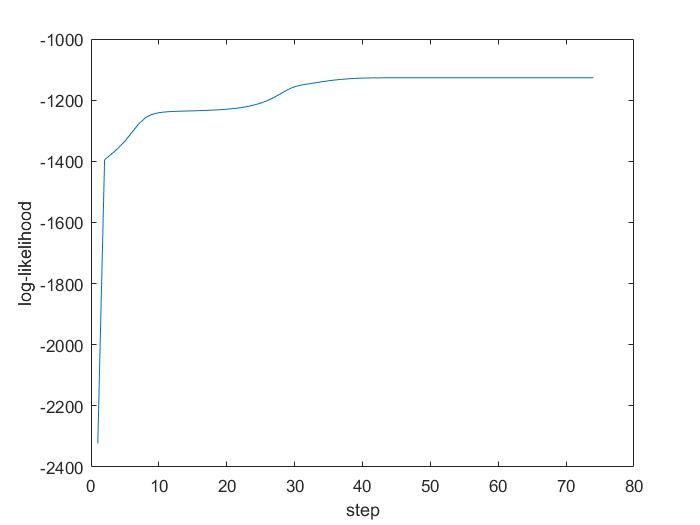
\includegraphics[scale=0.45]{figure1.jpg}\\
  {\footnotesize 图一 、   对数函数随着训练次数的变化曲线}\\
\end{figure}

2)根据实验结果得到,

$\pi_1 = 0.2935, \pi_2 = 0.4103, \pi_3 = 0.1472, \pi_4 = 0.1490$;

$\mu_1 = [-0.9911, -1.0074], \mu_2 = [0.9820, 1.0200], \mu_3 = [1.0402, -0.9899], \mu_4 = [-0.98, 1.0342]$;

${\sum}_1 = [0.2193, -0.0966; -0.0966, 0.1866], {\sum}_2 = [0.1558, -0.0750; -0.0750, 0.1594], {\sum}_3 = [0.2082, 0.0995; 0.0995, 0.1977], {\sum}_4 = [0.2319, 0.1044; 0.1044, 0.1958]$

将上述带入得到的参数带入式(3)中可得到GMM模型。

(3)从5000个点中随机抽取500个点,将相同类的点用相同的颜色表示,实验结果如下:
\begin{figure}[!htb]
  \centering
  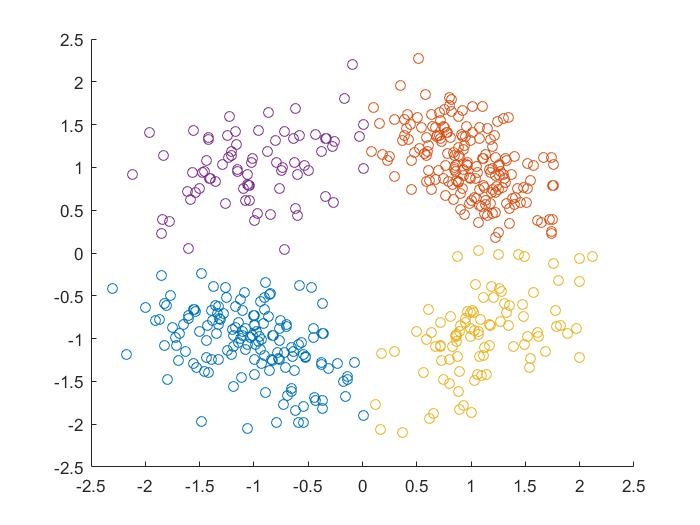
\includegraphics[scale=0.45]{figure2.jpg}\\
  {\footnotesize 图二 、   5000个数据点中随机抽取500个数据点}\\
\end{figure}

(4)EM算法参数的不同初始化方式会对收敛速度和收敛效果产生重要的影响,如果没有设置好初始值EM算法有可能会收敛于局部最小值而不能得到全局最优解。一般的初始化方法有随机中心、层次聚类和k-means等。在这里采用了随机中心的方法。

(5)EM算法是参数估计的重要方法,其核心是根据已有的数据来迭代计算似然函数,使之收敛于某个最优值。实验中还将所有5000个原始训练数据和经过GMM算法分类之后的数据点在二维图中表示出来如图三图四所示,由图可以发现应用随机中心算法在EM算法的收敛上表现优异。
\begin{figure}[!htb]
  \centering
  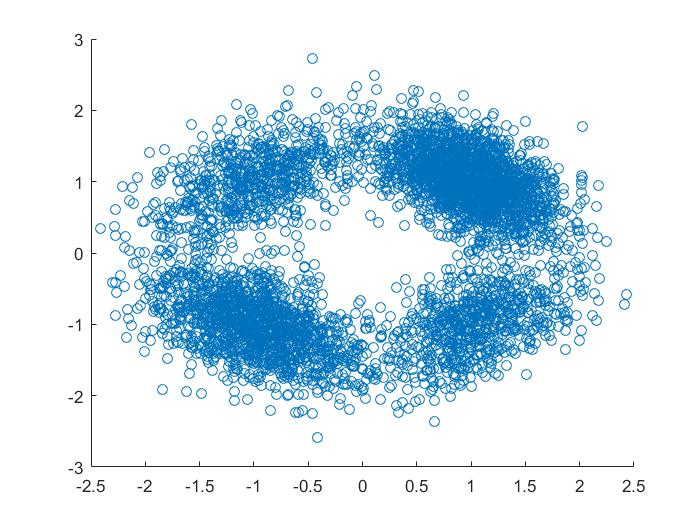
\includegraphics[scale=0.45]{3.jpg}\\
  {\footnotesize 图三、   5000个原始数据点}\\
\end{figure}

\begin{figure}[!htb]
  \centering
  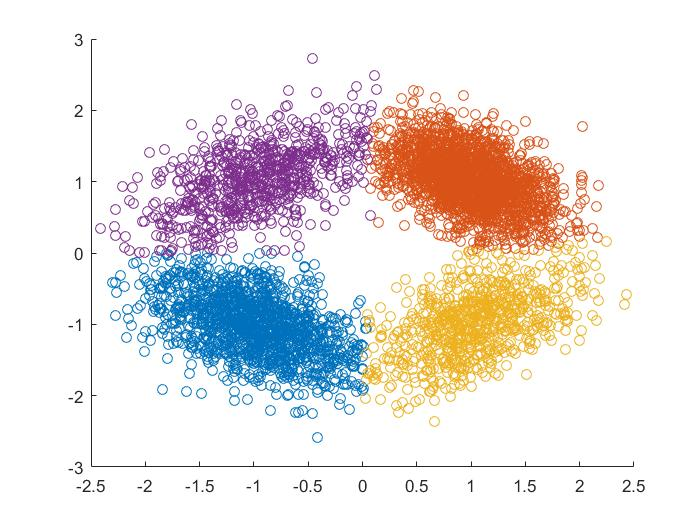
\includegraphics[scale=0.45]{4.jpg}\\
  {\footnotesize 图四 、   5000个分类之后的数据点}\\
\end{figure}















\end{document}
